\section{Idiotenseite}
\subsection{Ableitungen}
\begin{center}
	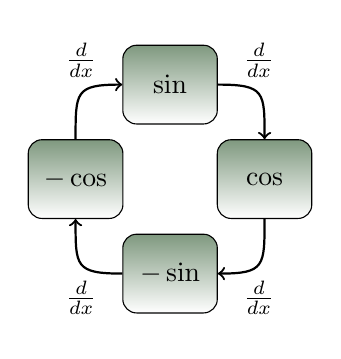
\begin{tikzpicture}
	[	inner sep = 2mm,
	sin/.style={rectangle,minimum width=1.2cm,minimum height=1cm,rounded corners=5pt,draw=black,top color=green!20!black!50},
	abl/.style={rectangle}
	]
	\node at (1.2,0) (sin1) [sin] {$\sin$};
	\node at (0,-1.2) (cos2) [sin] {$-\cos$};
	\node at (1.2,-2.4) (sin2) [sin] {$-\sin$};
	\node at (2.4,-1.2) (cos1) [sin] {$\cos$};
	
	\draw[thick,black,->] (sin1.east) .. controls +(right:0.6cm) and +(up:0.6cm) ..  (cos1.north)
	node [pos=0.5,above](abl) {$\frac{d}{dx}$};
	\draw[thick,black,->] (cos1.south) .. controls +(down:0.6cm) and +(right:0.6cm) .. (sin2.east)
	node [pos=0.5,below](abl) {$\frac{d}{dx}$};
	\draw[thick,black,->] (sin2.west) .. controls +(left:0.6cm) and +(down:0.6cm) .. (cos2.south)
	node [pos=0.5,below](abl) {$\frac{d}{dx}$};
	\draw[thick,black,->] (cos2.north) .. controls +(up:0.6cm) and +(left:0.6cm) .. (sin1.west)
	node [pos=0.5,above](abl) {$\frac{d}{dx}$};
\end{tikzpicture}
\end{center}

\subsection{Trigonometire}
\subsubsection{Einheitskreis}
\begin{center}
	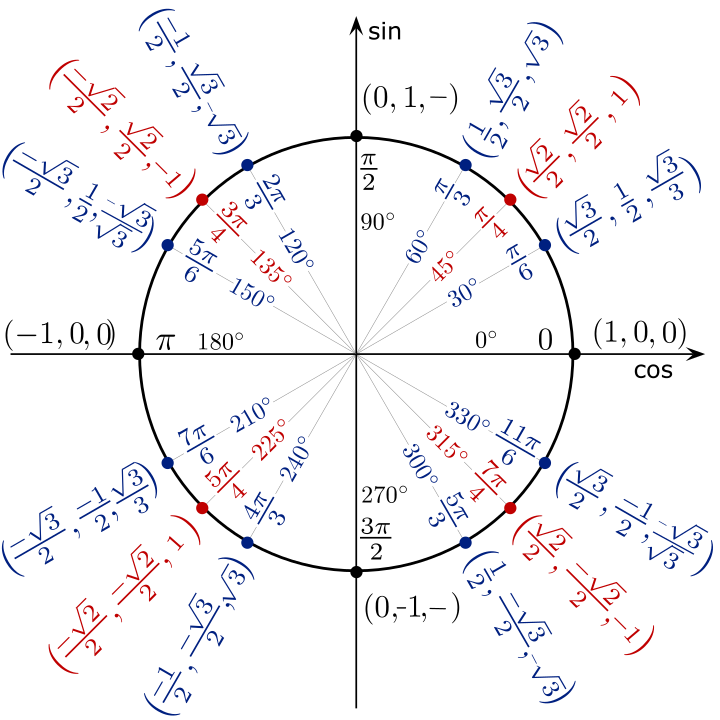
\includegraphics[width=0.8\columnwidth]{Images/einheitskreis}\\
	Punkte auf Kreis [$\cos(\alpha), \sin(\alpha), \tan(\alpha)$]
\end{center}

\subsubsection{Periodizität}
\begin{align*}
	\cos(a+k\cdot2\pi)=\cos(a) &\qquad \sin(a+k\cdot2\pi)=\sin(a) \qquad
(k \in \mathbb{Z})\\
\sin(-a\cdot t) = -\sin(a\cdot t)&\qquad 
\end{align*}

\subsubsection{Doppel- und Halbwinkel}	
\begin{align*}
	\sin(2a) &=2\sin(a)\cos(a) &= \frac{2\tan(a)}{1 +\tan^2(a)}\\
	\cos(2a) &=\cos^2(a)-\sin^2(a) &= 2\cos^2(a)-1 &= 1-2\sin^2(a)\\
	\cos^2 \left(\frac{a}{2}\right) &=\frac{1+\cos(a)}{2} \\
	\sin^2 \left(\dfrac{a}{2}\right)&=\frac{1-\cos(a)}{2}
\end{align*}


\subsubsection{Additionstheoreme}
\begin{align*}
	\sin(a \pm b)&=\sin(a) \cdot \cos(b) \pm \cos(a) \cdot \sin(b)\\
	\cos(a \pm b)&=\cos(a) \cdot \cos(b) \mp \sin(a) \cdot \sin(b)\\	
	\tan(a \pm b)&=\dfrac{\tan(a) \pm \tan(b)}{1 \mp \tan(a) \cdot \tan(b)}\\
	\sin(a)+\sin(b) &= 2\sin\left(\frac{a + b}{2}\right)\cos\left(\frac{a - b}{2}\right)\\
	\sin(a)-\sin(b) &= 2\cos\left(\frac{a + b}{2}\right)\sin\left(\frac{a - b}{2}\right)\\
	\cos(a)+\cos(b) &= 2\cos\left(\frac{a + b}{2}\right)\cos\left(\frac{a - b}{2}\right)\\
	\cos(a)-\cos(b) &= -2\sin\left(\frac{a + b}{2}\right)\sin\left(\frac{a - b}{2}\right)\\
	\sin(a)\sin(b)&=\frac{1}{2}(\cos(a-b)-\cos(a+b))\\
	\cos(a)\cos(b)&=\frac{1}{2}(\cos(a-b)+\cos(a+b))\\
	\sin(a)\cos(b)&=\frac{1}{2}(\sin(a-b)+\sin(a+b))\\
\end{align*}

\subsubsection{Potenzen}
\begin{align*}
	\sin^2(a) &= \frac{1}{2}(1 - \cos(2a)) \\
	\sin^3(a) &= \frac{1}{4}(3\sin(a) - \sin(3a)) \\
	\cos^2(a) &= \frac{1}{2}(1 + \cos(2a)) \\
	\cos^3(a) &= \frac{1}{4}(3\cos(a) + \cos(3a)) \\
\end{align*}

\subsection{Partialbruchzerlegung}
Summanden einzeln bewerten:
\begin{itemize}[nosep]
	\item einfachen Nullstellen: $\frac{x+1}{x^2 - 3x +2} \rightarrow \frac{A}{x-1} + \frac{B}{x-2}$
	\item mehrfach Nullstellen: $\frac{x+1}{x^2 + 2x +1} \rightarrow \frac{A}{(x+1)}+\frac{B}{(x+1)^2}$
	\item komplexe Nullstellen: $\frac{x+1}{x^2 + 1} \rightarrow \frac{Ax + B}{x^2 + 1}$
\end{itemize}
